In this section, we discuss the offline performance of \pred\ when the number of tasks $\Mpr \gg A \geq n$.

We first discuss how \pred\ (\gt) is modified for the offline setting. 
%
In the offline setting, the \pred\ first samples a task $m\sim\cTs$, then the test dataset $\H_m\sim \Dts(\cdot|m)$. Then \pred\ and \predt\ act similarly to the online setting, but based on the entire offline dataset $\H_m$. 
% and acts greedily. That is, at every round $t$, 
%
The full pseudocode of \pred\ is in \Cref{alg:pred-off}.

\begin{algorithm}[!tbh]
\caption{\textbf{Pre}-trained \textbf{De}cision \textbf{T}ransf\textbf{o}rmer with \textbf{R}eward Estimation (\pred)}
\label{alg:pred-off}
    \begin{algorithmic}[1]
    \STATE \textbf{Collecting Pretraining Dataset} 
    \STATE Initialize empty pretraining dataset $\Htr$
    \FOR{$i$ in $[\Mpr]$ }
    \STATE Sample task $m \sim \cTp$, in-context dataset $\H_m \sim \Dpr(\cdot | m)$ and add this to $\Htr$.
    \ENDFOR
    \STATE \textbf{Pretraining model on dataset}
    \STATE Initialize model $\T_{\bTheta}$ with parameters $\bTheta$
    \WHILE{\text{not converged}}
    \STATE Sample $\H_m$ from $\Htr$ and predict $\wr_{m,t}$ for action $(I_{m,t})$ for all $t \in[n]$
    \STATE Compute loss in \eqref{eq:loss-transformer} with respect to $r_{m,t}$ and backpropagate to update model parameter $\bTheta$.
    \ENDWHILE
    \STATE \textbf{Offline test-time deployment}
    \STATE Sample unknown task $m \sim \cTs$, sample dataset $\H_m \sim \Dts(\cdot | m)$
    \STATE Use $\T_{\bTheta}$ on $m$ at round $t$ to choose 
    \begin{align*}
        I_t \begin{cases}
            = \argmax_{a\in\A} \T_{\bTheta}\left( \wr_{m,t}(a) \mid \H_m\right), & \textbf{\pred} \\
            %%%%%%%%%%%%%%%%%%%%%%%
            \sim \textrm{softmax}^\tau_a \T_{\bTheta}\left( \wr_{m,t}(a) \mid \H_m\right), & \textbf{\predt}
        \end{cases}
    \end{align*}
    % %
    % \STATE \textbf{Online test-time deployment}
    % \STATE Sample unknown task $m \sim \cTs$ and initialize empty $\H_m^{0}=\{\emptyset\}$
    % \FOR{$t=1,2,\ldots,n$}
    % \STATE Use $\T_{\bTheta}$ on $m$ at round $t$ to choose 
    % \begin{align*}
    %     I_t \begin{cases}
    %         = \argmax_{a\in\A} \T_{\bTheta}\left( \wr_{m,t}(a) \mid \H^t_m\right), & \textbf{\pred} \\
    %         %%%%%%%%%%%%%%%%%%%%%%%
    %         \sim \textrm{softmax}^\tau_a \T_{\bTheta}\left( \wr_{m,t}(a) \mid \H^t_m\right), & \textbf{\predt}
    %     \end{cases}
    % \end{align*}
    % %
    % % $I_t = \argmax_{a\in\A} \T_{\bTheta}\left( \wr_{m,t}(a) \mid \H^t_m\right)$ and observe $r_t$
    % \STATE Add $\left\{I_t, r_t\right\}$ to $\H_m^t$
    % \ENDFOR
    \end{algorithmic}
\end{algorithm}








Recall that $\Dts$ denote a distribution over all possible interactions that can be generated by $\pi^w$ during test time. 
%
%
%
%
For offline testing, first, a test task $m\sim\cTs$, and then an in-context test dataset $\H_m$ is collected such that $\H_m\sim\Dts(\cdot|m)$. 
% The policy that the model in-context learns is given conditionally as $\T_{\bTheta}(\cdot \mid \H_m)$. So we evaluate the policy by selecting action $I_t \in \argmax_a \T_{\bTheta}\left(a \mid \H_m\right)$. 
%
% 
Observe from \Cref{alg:pred-off} that in the offline setting, \pred\ first samples a task $m\sim\cTs$, and then a test dataset $\H_m\sim \Dts(\cdot|m)$ and acts greedily. 
%
Crucially in the offline setting the 
% That is, at every round $t$, \pred\ chooses $I_t = \argmax_{a\in\A_m} \T_\bw\left( \wr_{m,t}(a) \mid \H_m\right)$ which is the action with the highest predicted reward and $\wr_{m,t}(a)$ is the predicted reward of action $a$. Also, observe that 
\pred\ does not add the observed reward $r_t$ at round $t$ to the dataset.
%
Through this experiment, we want to evaluate the performance of \pred\ to learn the underlying latent structure and reward correlation when the horizon is small.
%
Finally, recall that when the horizon is small the weak demonstrator $\pi^w$ does not have sufficient samples for each action. This leads to a poor approximation of the greedy action. 


%
% In offline setting, the dataset $\H_m$ is sampled before and is not altered.


\textbf{Baselines:} We again implement the same baselines discussed in \Cref{sec:short-horizon}. The baselines are \pred, \predt, \dptg, \ad, \ts, and \linucb. During test time evaluation for offline setting the \dpt\ selects $I_t =  \widehat{a}_{m,t,*}$ where $\widehat{a}_{m,t,*} = \argmax_a \T_{\bTheta}(a|\H^t_m)$ is the predicted optimal action. 


\textbf{Outcomes:} We first discuss the main outcomes of our experimental results for increasing the horizon:

\begin{tcolorbox}
\customfinding  \pred\ (\gt) performs comparably to \dptg\ and \ad\ in the offline setting. 
\end{tcolorbox}

% \noindent
% \textbf{(1)} The \pred\ performs comparably with respect to cumulative regret against \dptg\ both for the long horizon and the short horizon setting. 

% \textbf{(2)} The \pred\ performs comparably with respect to cumulative regret against \dptg\ both for the linear and the non-linear bandit setting.

% \textbf{(3)} The \pred\ and \dptg\ has comparable regret to the weak demonstrator \ts\ and \linucb\ in the offline setting.





% \begin{figure}[!hbt]
% \centering
% \begin{tabular}{cc}
% % \subfigure[Offline for long horizon]{\hspace*{-1.5em}\includegraphics[scale = 0.1]{img/final/offline/off_large_lr0.00015_do0_embd32_layer4_head4_envs200006_hists1_samples1_var0.3_cov0.0_H50_d20_lind5_seed1_testcov0.0_hor50.pkl_bar copy.png}\label{fig:off-large}} &
% % %%%%%%%%%%
% % \hspace*{-1.5em}\subfigure[Offline for short horizon]{\includegraphics[scale = 0.1]{img/final/offline/off_small_lr0.00015_do0_embd32_layer4_head4_envs120000_hists1_samples1_var0.3_cov0.0_H50_d10_lind2_seed1_testcov0.0_hor50.pkl_bar.png} \label{fig:off-small}} &
% %%%%%%%%%%%%%%%%%%%%%%%
% \subfigure[Offline for Linear setting]{\hspace*{-1.5em}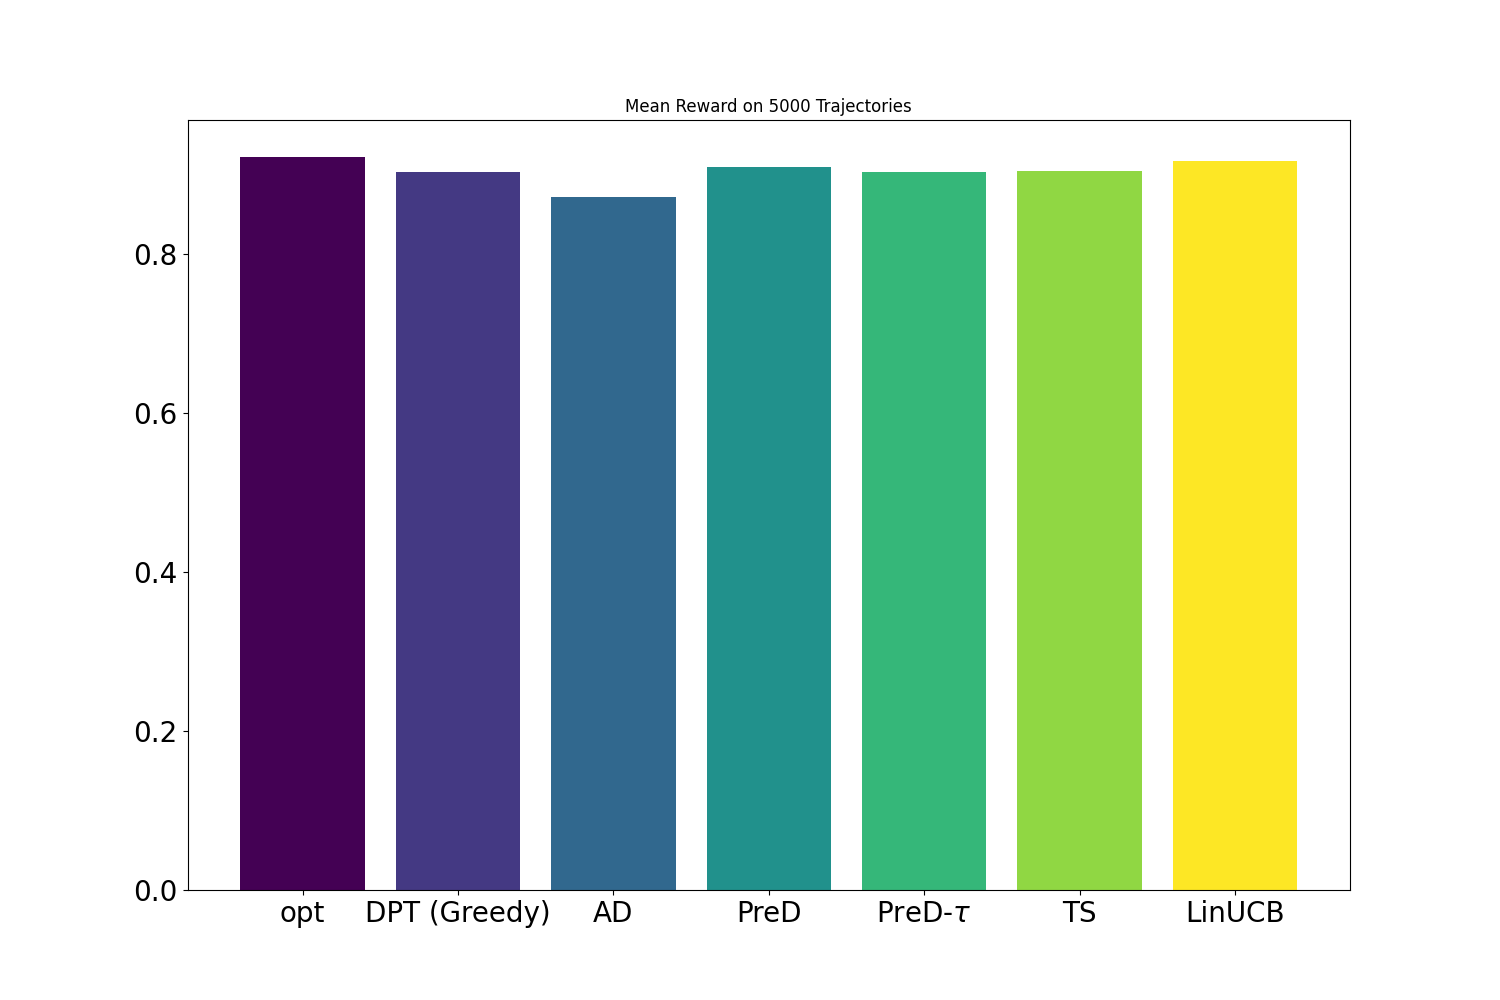
\includegraphics[scale = 0.15]{img/Neurips/offline/lin_off_lr0.00015_do0_embd32_layer4_head4_envs120000_hists1_samples1_var0.3_cov0.0_H50_d10_lind2_seed1_testcov0.0_hor50.pkl_bar.png}\label{fig:off-lin-small}} &
% %%%%%%%%%%
% \hspace*{-1.5em}\subfigure[Offline for Non-linear setting]{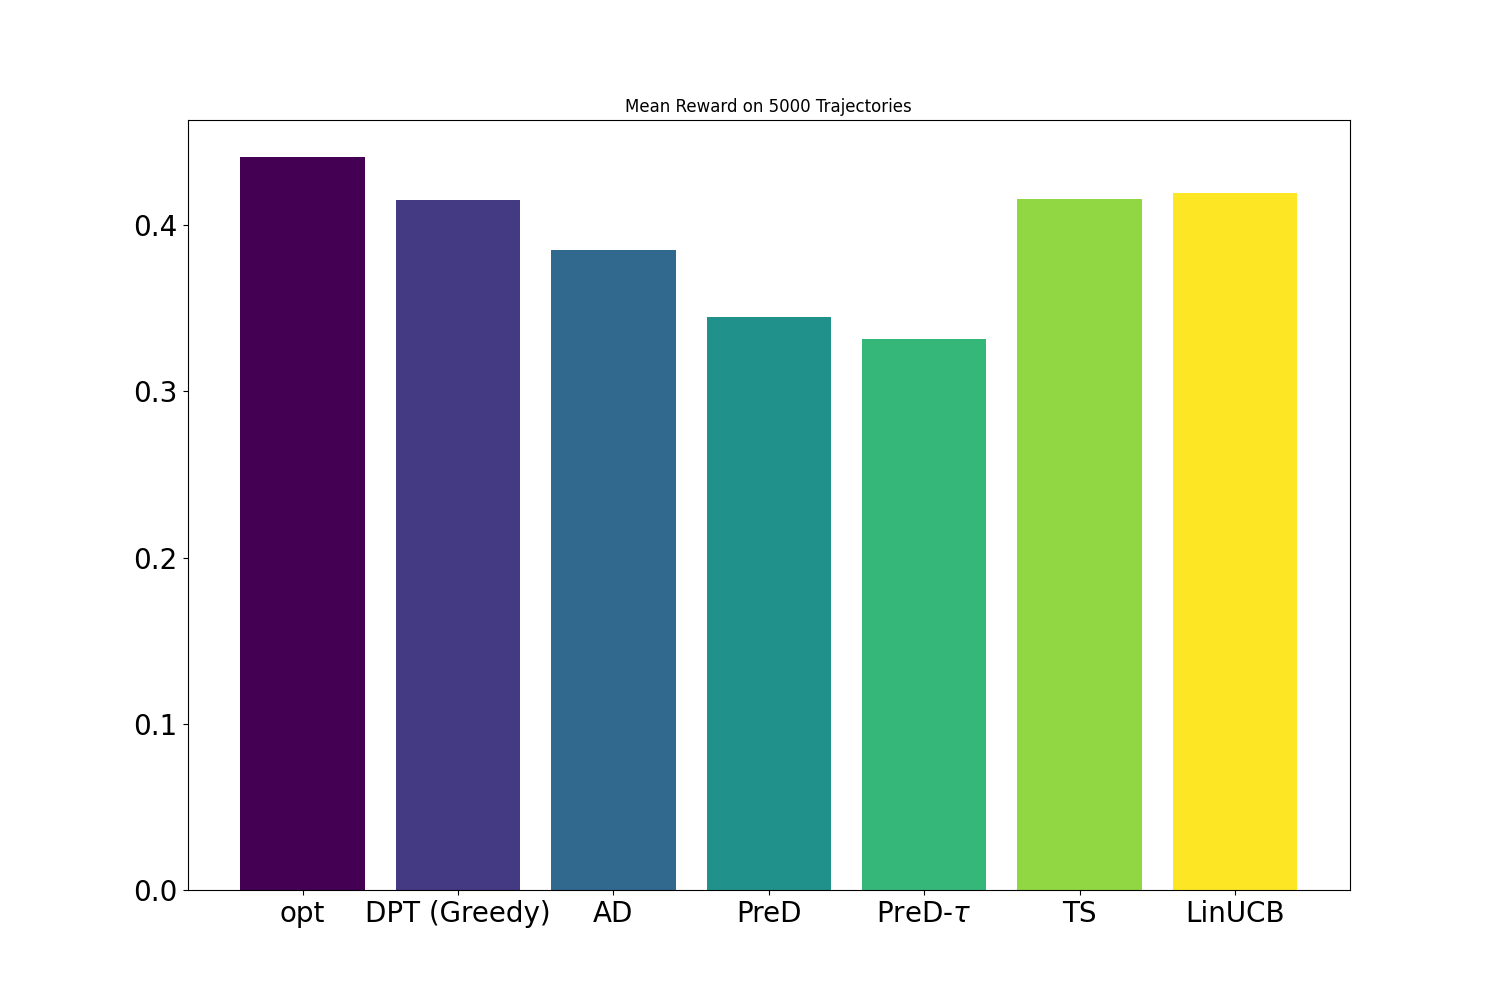
\includegraphics[scale = 0.15]{img/Neurips/offline/nlm_off_lr0.00015_do0_embd32_layer4_head4_envs120001_hists1_samples1_var0.3_cov0.0_H50_d6_lind2_seed1_testcov0.0_hor50.pkl_bar.png} \label{fig:off-lin-large}}
% \end{tabular}
% \vspace*{-1em}
% \caption{Offline experiment. The y-axis shows the cumulative reward.}
% \label{fig:expt-offline}
% \vspace{-0.7em}
% \end{figure}

\begin{figure}[!hbt]
\centering
\vspace*{-1em}
\begin{subfigure}[b]{0.48\textwidth}
   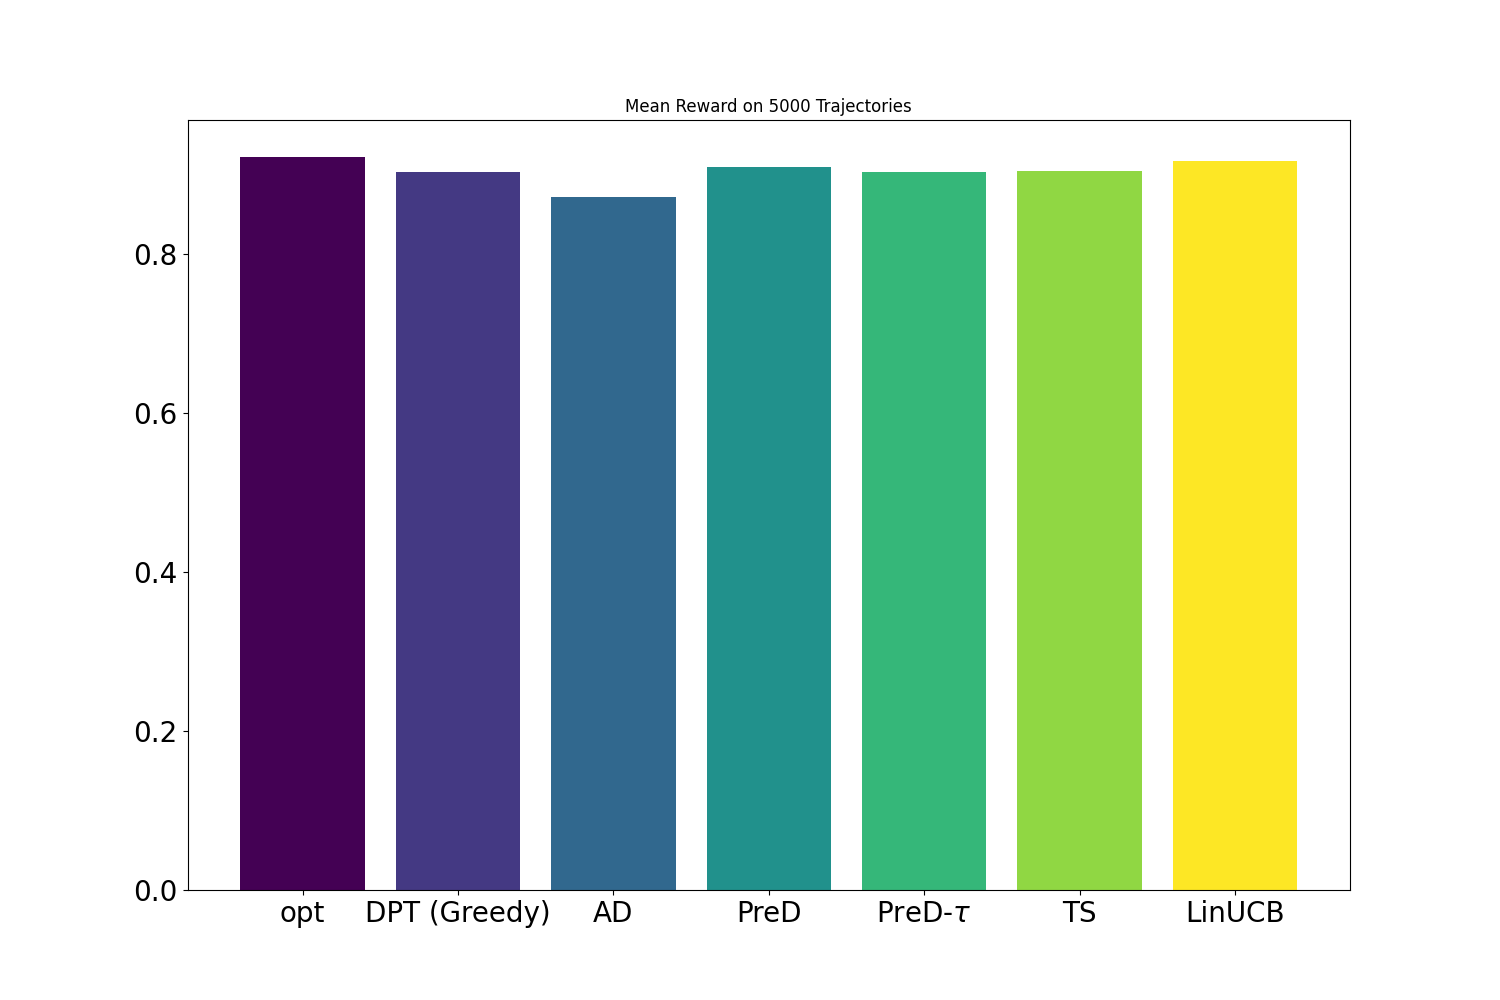
\includegraphics[scale=0.15]{img/Neurips/offline/lin_off_lr0.00015_do0_embd32_layer4_head4_envs120000_hists1_samples1_var0.3_cov0.0_H50_d10_lind2_seed1_testcov0.0_hor50.pkl_bar.png}
   \caption{Offline for Linear setting}
   \label{fig:off-lin-small}
\end{subfigure}%
\begin{subfigure}[b]{0.48\textwidth}
   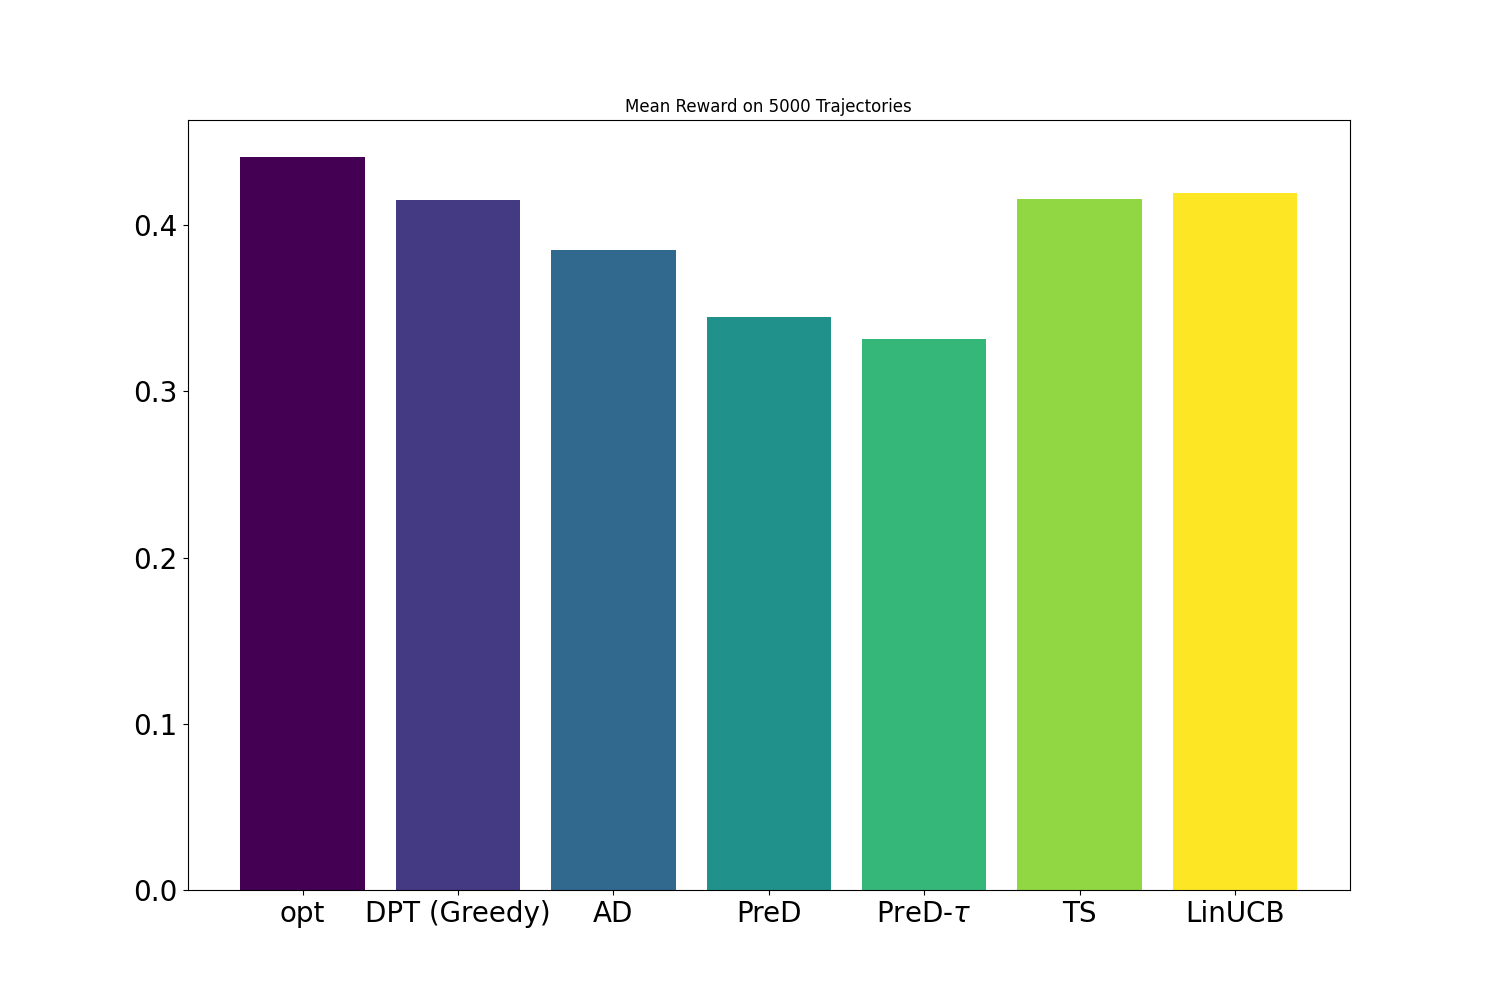
\includegraphics[scale=0.15]{img/Neurips/offline/nlm_off_lr0.00015_do0_embd32_layer4_head4_envs120001_hists1_samples1_var0.3_cov0.0_H50_d6_lind2_seed1_testcov0.0_hor50.pkl_bar.png}
   \caption{Offline for Non-linear setting}
   \label{fig:off-lin-large}
\end{subfigure}
\vspace*{-1em}
\caption{Offline experiment. The y-axis shows the cumulative reward.}
\label{fig:expt-offline}
\vspace{-0.7em}
\end{figure}

\textbf{Experimental Result:} We observe these outcomes in \Cref{fig:expt-offline}. In \Cref{fig:expt-offline} we show the linear bandit setting for horizon $n=20$, $\Mpr =  200000$, $\Mts = 5000$, $A=20$, and $d=5$ for the low data regime.
% and $n=40$ for long horizon respectively.
%
%
Again, the demonstrator $\pi^w$ is the \ts\ algorithm. We observe that \pred\ (\gt) has comparable cumulative regret to \dptg. Note that for any task $m$ for the horizon $n=20$ the \ts\ will be able to sample all the actions at most once. 
% We can observe the result in \Cref{fig:off-large}, and \ref{fig:off-small}.
% Moreover \pred\ matches the performance of \linucb. 
%
%
% In the linear setting of \cref{fig:off-lin-small} the number of offline tasks is small, such that  $\Mts = 200$. The remaining parameters are the same as the offline experiment discussed before.
%
In the non-linear setting of \Cref{fig:off-lin-large} the $n=40$, $\Mpr =  100000$, $A=6$, $d=2$.
%
Observe that in all of these results, the performance of \pred\ (\gt) is comparable with respect to cumulative regret against \dptg.




